\documentclass[]{article}
\usepackage{lmodern}
\usepackage{amssymb,amsmath}
\usepackage{ifxetex,ifluatex}
\usepackage{fixltx2e} % provides \textsubscript
\ifnum 0\ifxetex 1\fi\ifluatex 1\fi=0 % if pdftex
  \usepackage[T1]{fontenc}
  \usepackage[utf8]{inputenc}
\else % if luatex or xelatex
  \ifxetex
    \usepackage{mathspec}
  \else
    \usepackage{fontspec}
  \fi
  \defaultfontfeatures{Ligatures=TeX,Scale=MatchLowercase}
\fi
% use upquote if available, for straight quotes in verbatim environments
\IfFileExists{upquote.sty}{\usepackage{upquote}}{}
% use microtype if available
\IfFileExists{microtype.sty}{%
\usepackage{microtype}
\UseMicrotypeSet[protrusion]{basicmath} % disable protrusion for tt fonts
}{}
\usepackage[margin=1in]{geometry}
\usepackage{hyperref}
\hypersetup{unicode=true,
            pdftitle={Tourism Data Analysis},
            pdfborder={0 0 0},
            breaklinks=true}
\urlstyle{same}  % don't use monospace font for urls
\usepackage{color}
\usepackage{fancyvrb}
\newcommand{\VerbBar}{|}
\newcommand{\VERB}{\Verb[commandchars=\\\{\}]}
\DefineVerbatimEnvironment{Highlighting}{Verbatim}{commandchars=\\\{\}}
% Add ',fontsize=\small' for more characters per line
\usepackage{framed}
\definecolor{shadecolor}{RGB}{248,248,248}
\newenvironment{Shaded}{\begin{snugshade}}{\end{snugshade}}
\newcommand{\KeywordTok}[1]{\textcolor[rgb]{0.13,0.29,0.53}{\textbf{#1}}}
\newcommand{\DataTypeTok}[1]{\textcolor[rgb]{0.13,0.29,0.53}{#1}}
\newcommand{\DecValTok}[1]{\textcolor[rgb]{0.00,0.00,0.81}{#1}}
\newcommand{\BaseNTok}[1]{\textcolor[rgb]{0.00,0.00,0.81}{#1}}
\newcommand{\FloatTok}[1]{\textcolor[rgb]{0.00,0.00,0.81}{#1}}
\newcommand{\ConstantTok}[1]{\textcolor[rgb]{0.00,0.00,0.00}{#1}}
\newcommand{\CharTok}[1]{\textcolor[rgb]{0.31,0.60,0.02}{#1}}
\newcommand{\SpecialCharTok}[1]{\textcolor[rgb]{0.00,0.00,0.00}{#1}}
\newcommand{\StringTok}[1]{\textcolor[rgb]{0.31,0.60,0.02}{#1}}
\newcommand{\VerbatimStringTok}[1]{\textcolor[rgb]{0.31,0.60,0.02}{#1}}
\newcommand{\SpecialStringTok}[1]{\textcolor[rgb]{0.31,0.60,0.02}{#1}}
\newcommand{\ImportTok}[1]{#1}
\newcommand{\CommentTok}[1]{\textcolor[rgb]{0.56,0.35,0.01}{\textit{#1}}}
\newcommand{\DocumentationTok}[1]{\textcolor[rgb]{0.56,0.35,0.01}{\textbf{\textit{#1}}}}
\newcommand{\AnnotationTok}[1]{\textcolor[rgb]{0.56,0.35,0.01}{\textbf{\textit{#1}}}}
\newcommand{\CommentVarTok}[1]{\textcolor[rgb]{0.56,0.35,0.01}{\textbf{\textit{#1}}}}
\newcommand{\OtherTok}[1]{\textcolor[rgb]{0.56,0.35,0.01}{#1}}
\newcommand{\FunctionTok}[1]{\textcolor[rgb]{0.00,0.00,0.00}{#1}}
\newcommand{\VariableTok}[1]{\textcolor[rgb]{0.00,0.00,0.00}{#1}}
\newcommand{\ControlFlowTok}[1]{\textcolor[rgb]{0.13,0.29,0.53}{\textbf{#1}}}
\newcommand{\OperatorTok}[1]{\textcolor[rgb]{0.81,0.36,0.00}{\textbf{#1}}}
\newcommand{\BuiltInTok}[1]{#1}
\newcommand{\ExtensionTok}[1]{#1}
\newcommand{\PreprocessorTok}[1]{\textcolor[rgb]{0.56,0.35,0.01}{\textit{#1}}}
\newcommand{\AttributeTok}[1]{\textcolor[rgb]{0.77,0.63,0.00}{#1}}
\newcommand{\RegionMarkerTok}[1]{#1}
\newcommand{\InformationTok}[1]{\textcolor[rgb]{0.56,0.35,0.01}{\textbf{\textit{#1}}}}
\newcommand{\WarningTok}[1]{\textcolor[rgb]{0.56,0.35,0.01}{\textbf{\textit{#1}}}}
\newcommand{\AlertTok}[1]{\textcolor[rgb]{0.94,0.16,0.16}{#1}}
\newcommand{\ErrorTok}[1]{\textcolor[rgb]{0.64,0.00,0.00}{\textbf{#1}}}
\newcommand{\NormalTok}[1]{#1}
\usepackage{graphicx,grffile}
\makeatletter
\def\maxwidth{\ifdim\Gin@nat@width>\linewidth\linewidth\else\Gin@nat@width\fi}
\def\maxheight{\ifdim\Gin@nat@height>\textheight\textheight\else\Gin@nat@height\fi}
\makeatother
% Scale images if necessary, so that they will not overflow the page
% margins by default, and it is still possible to overwrite the defaults
% using explicit options in \includegraphics[width, height, ...]{}
\setkeys{Gin}{width=\maxwidth,height=\maxheight,keepaspectratio}
\IfFileExists{parskip.sty}{%
\usepackage{parskip}
}{% else
\setlength{\parindent}{0pt}
\setlength{\parskip}{6pt plus 2pt minus 1pt}
}
\setlength{\emergencystretch}{3em}  % prevent overfull lines
\providecommand{\tightlist}{%
  \setlength{\itemsep}{0pt}\setlength{\parskip}{0pt}}
\setcounter{secnumdepth}{0}
% Redefines (sub)paragraphs to behave more like sections
\ifx\paragraph\undefined\else
\let\oldparagraph\paragraph
\renewcommand{\paragraph}[1]{\oldparagraph{#1}\mbox{}}
\fi
\ifx\subparagraph\undefined\else
\let\oldsubparagraph\subparagraph
\renewcommand{\subparagraph}[1]{\oldsubparagraph{#1}\mbox{}}
\fi

%%% Use protect on footnotes to avoid problems with footnotes in titles
\let\rmarkdownfootnote\footnote%
\def\footnote{\protect\rmarkdownfootnote}

%%% Change title format to be more compact
\usepackage{titling}

% Create subtitle command for use in maketitle
\providecommand{\subtitle}[1]{
  \posttitle{
    \begin{center}\large#1\end{center}
    }
}

\setlength{\droptitle}{-2em}

  \title{Tourism Data Analysis}
    \pretitle{\vspace{\droptitle}\centering\huge}
  \posttitle{\par}
    \author{}
    \preauthor{}\postauthor{}
      \predate{\centering\large\emph}
  \postdate{\par}
    \date{31 July 2019}

\usepackage{booktabs}
\usepackage{longtable}
\usepackage{array}
\usepackage{multirow}
\usepackage{wrapfig}
\usepackage{float}
\usepackage{colortbl}
\usepackage{pdflscape}
\usepackage{tabu}
\usepackage{threeparttable}
\usepackage{threeparttablex}
\usepackage[normalem]{ulem}
\usepackage{makecell}
\usepackage{xcolor}

\begin{document}
\maketitle

\section{BoxCox Transformation}\label{boxcox-transformation}

\begin{tabular}{l|r|r|r}
\hline
R.method & Bias & Unbiased (Method 1) & Unbiased (Method 2)\\
\hline
Base & 12.27 & 139.94 & 13.45\\
\hline
Bottom-up & 18.06 & 15.76 & 23.33\\
\hline
MinT(Shrink) & 10.27 & 10.11 & 12.43\\
\hline
OLS & 11.84 & 116.91 & 12.96\\
\hline
WLS & 15.83 & 14.20 & 19.51\\
\hline
\end{tabular}

\section{More analysis on BoxCox transformed
resulst}\label{more-analysis-on-boxcox-transformed-resulst}

\begin{Shaded}
\begin{Highlighting}[]
\NormalTok{DF_BoxCoxTrans }\OperatorTok\StringTok{ }
\StringTok{  }\KeywordTok{group_by}\NormalTok{(}\StringTok{`}\DataTypeTok{F.method}\StringTok{`}\NormalTok{, }\StringTok{`}\DataTypeTok{R.method}\StringTok{`}\NormalTok{, Forecast_Horizon, Series) }\OperatorTok\StringTok{ }
\StringTok{  }\KeywordTok{summarise}\NormalTok{(}\DataTypeTok{MSE =} \KeywordTok{round}\NormalTok{(}\KeywordTok{mean}\NormalTok{(SquaredE)}\OperatorTok{/}\FloatTok{1e3}\NormalTok{, }\DataTypeTok{digits =} \DecValTok{2}\NormalTok{)) }\OperatorTok\StringTok{ }
\StringTok{  }\KeywordTok{filter}\NormalTok{(R.method }\OperatorTok{==}\StringTok{ "Base"}\NormalTok{, Forecast_Horizon }\OperatorTok{==}\StringTok{ }\DecValTok{1}\NormalTok{, }
\NormalTok{         F.method }\OperatorTok\KeywordTok{c}\NormalTok{(}\StringTok{"Bias"}\NormalTok{,}\StringTok{"Unbiased_M1"}\NormalTok{)) }\OperatorTok\StringTok{ }
\StringTok{  }\KeywordTok{ungroup}\NormalTok{() }\OperatorTok\StringTok{ }
\StringTok{  }\NormalTok{dplyr}\OperatorTok{::}\KeywordTok{select}\NormalTok{(}\OperatorTok{-}\NormalTok{R.method, }\OperatorTok{-}\NormalTok{Forecast_Horizon) }\OperatorTok\StringTok{ }
\StringTok{  }\KeywordTok{spread}\NormalTok{(}\DataTypeTok{key =}\NormalTok{ F.method, }\DataTypeTok{value =}\NormalTok{ MSE) }\OperatorTok\StringTok{ }
\StringTok{  }\KeywordTok{mutate}\NormalTok{(}\StringTok{"Bias-Unbiase"}\NormalTok{ =}\StringTok{ }\NormalTok{Bias }\OperatorTok{-}\StringTok{ }\NormalTok{Unbiased_M1) }\OperatorTok\StringTok{ }
\StringTok{  }\KeywordTok{filter}\NormalTok{(}\StringTok{`}\DataTypeTok{Bias-Unbiase}\StringTok{`} \OperatorTok{<}\StringTok{ }\OperatorTok{-}\DecValTok{5}\NormalTok{)}
\end{Highlighting}
\end{Shaded}

\begin{verbatim}
## # A tibble: 1 x 4
##   Series  Bias Unbiased_M1 `Bias-Unbiase`
##   <fct>  <dbl>       <dbl>          <dbl>
## 1 Total   808.      14866.        -14058.
\end{verbatim}

Bias correction is giving wiered results for \texttt{Total} series.

\begin{Shaded}
\begin{Highlighting}[]
\NormalTok{DF_BoxCoxTrans }\OperatorTok\StringTok{ }
\StringTok{  }\KeywordTok{filter}\NormalTok{(Forecast_Horizon }\OperatorTok{==}\StringTok{ }\DecValTok{1}\NormalTok{) ->}\StringTok{ }\NormalTok{DF_BoxCoxTrans_h1}

\NormalTok{DF_BoxCoxTrans_h1 }\OperatorTok\StringTok{ }
\StringTok{  }\KeywordTok{filter}\NormalTok{(Series }\OperatorTok{==}\StringTok{ "Total"}\NormalTok{, R.method }\OperatorTok{==}\StringTok{ "Base"}\NormalTok{, F.method }\OperatorTok{==}\StringTok{ "Bias"}\NormalTok{) }\OperatorTok\StringTok{ }
\StringTok{  }\NormalTok{dplyr}\OperatorTok{::}\KeywordTok{select}\NormalTok{(Actual, Replication) ->}\StringTok{ }\NormalTok{Total_True}
  
  
\NormalTok{DF_BoxCoxTrans_h1 }\OperatorTok\StringTok{ }
\StringTok{  }\KeywordTok{filter}\NormalTok{(Series }\OperatorTok{==}\StringTok{ "Total"}\NormalTok{, R.method }\OperatorTok{==}\StringTok{ "Base"}\NormalTok{, F.method }\OperatorTok\KeywordTok{c}\NormalTok{(}\StringTok{"Bias"}\NormalTok{,}\StringTok{"Unbiased_M1"}\NormalTok{)) ->}\StringTok{ }\NormalTok{Total_Fc}


\KeywordTok{ggplot}\NormalTok{() }\OperatorTok{+}\StringTok{ }
\StringTok{  }\KeywordTok{geom_line}\NormalTok{(}\DataTypeTok{data =}\NormalTok{ Total_Fc, }\KeywordTok{aes}\NormalTok{(}\DataTypeTok{x =}\NormalTok{ Replication, }\DataTypeTok{y =}\NormalTok{ Forecasts, }\DataTypeTok{color =} \StringTok{`}\DataTypeTok{F.method}\StringTok{`}\NormalTok{)) }\OperatorTok{+}\StringTok{ }
\StringTok{  }\KeywordTok{geom_line}\NormalTok{(}\DataTypeTok{data =}\NormalTok{ Total_True, }\DataTypeTok{mapping =} \KeywordTok{aes}\NormalTok{(}\DataTypeTok{x =}\NormalTok{ Replication, }\DataTypeTok{y =}\NormalTok{ Actual)) }\OperatorTok{+}\StringTok{ }
\StringTok{    }\KeywordTok{ylab}\NormalTok{(}\StringTok{"Forecasts/True"}\NormalTok{)}
\end{Highlighting}
\end{Shaded}

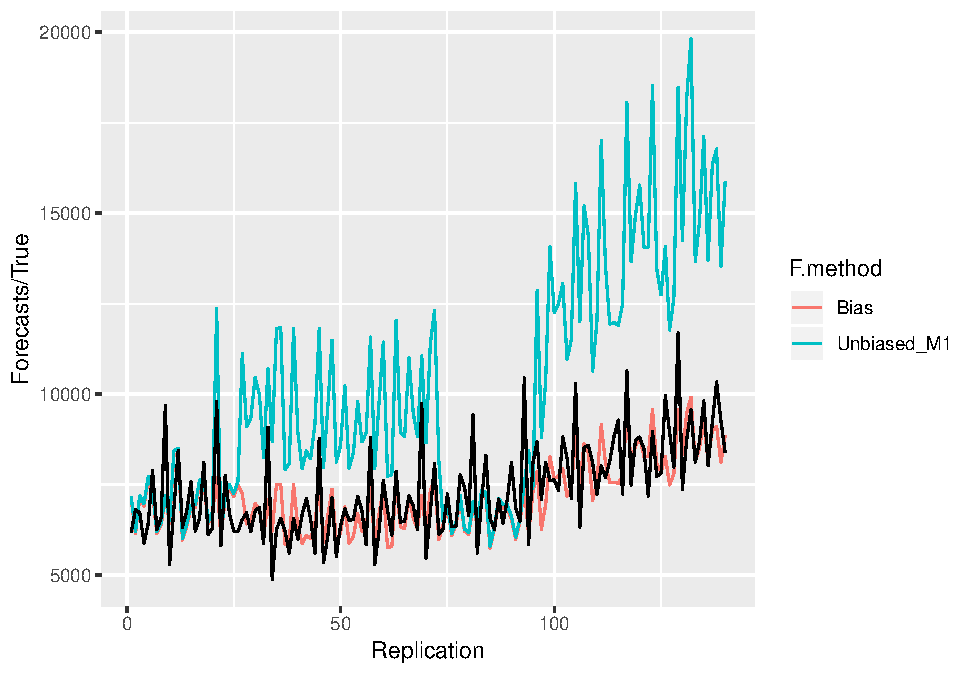
\includegraphics{TourismData-Final-results_files/figure-latex/unnamed-chunk-3-1.pdf}

\section{Log Transformation}\label{log-transformation}

\begin{tabular}{l|r|r|r}
\hline
R.method & Bias & Unbiased (Method 1) & Unbiased (Method 2)\\
\hline
Base & 12.06 & 11.87 & 12.52\\
\hline
Bottom-up & 17.37 & 15.47 & 21.58\\
\hline
MinT(Shrink) & 9.36 & 9.25 & 10.35\\
\hline
OLS & 11.59 & 11.41 & 11.98\\
\hline
WLS & 15.00 & 13.83 & 17.55\\
\hline
\end{tabular}

\begin{verbatim}
## Adding missing grouping variables: `F.method`
\end{verbatim}

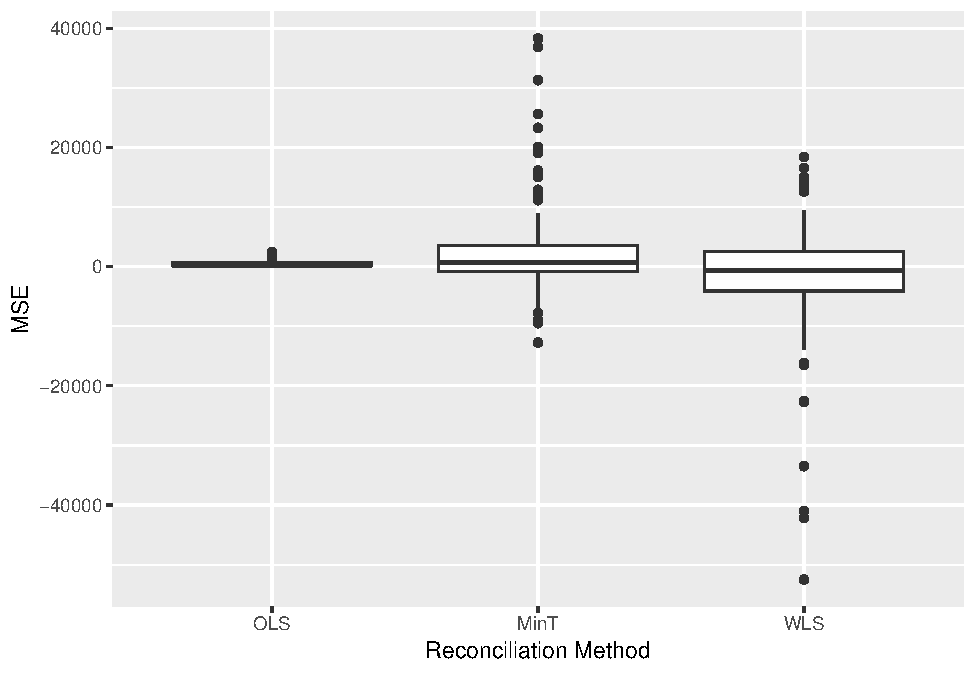
\includegraphics{TourismData-Final-results_files/figure-latex/unnamed-chunk-5-1.pdf}


\end{document}
